\section{校区环境}

北邮现在使用中的校区一共两个,即西土城路校区(海淀区,本部)和沙河校区(昌平区)。\footnote{另有西城区小西天校区(校舍)和昌平区宏福校区(接近弃用),目前和大家关系不大}校本部位于海淀区西土城路10号,面积很小,住宿条件相对较差,但交通便利,对面就是北师大,周围没事众多。目前,大三大四的本科生及多数研究生在本部学习。沙河校区是新生入学的校区,位于昌平区沙河镇南丰路{\small{}与高教园南三街交口向北400米路东(我知道写这些你不会看的)}。规划面积很大(大概本部三倍)但是实际建成只有一半左右,住宿学习环境好,但比较偏僻,被两个地铁站夹在中间导致出行不便。沙河校区主要容纳大一大二学生。

按照学校最新的安排,计算机学院包括软工在内的学生都将只在沙河待一年,大二的时候就会搬到本部,所以今年沙河就只有22级的新生啦。

\begin{center}
    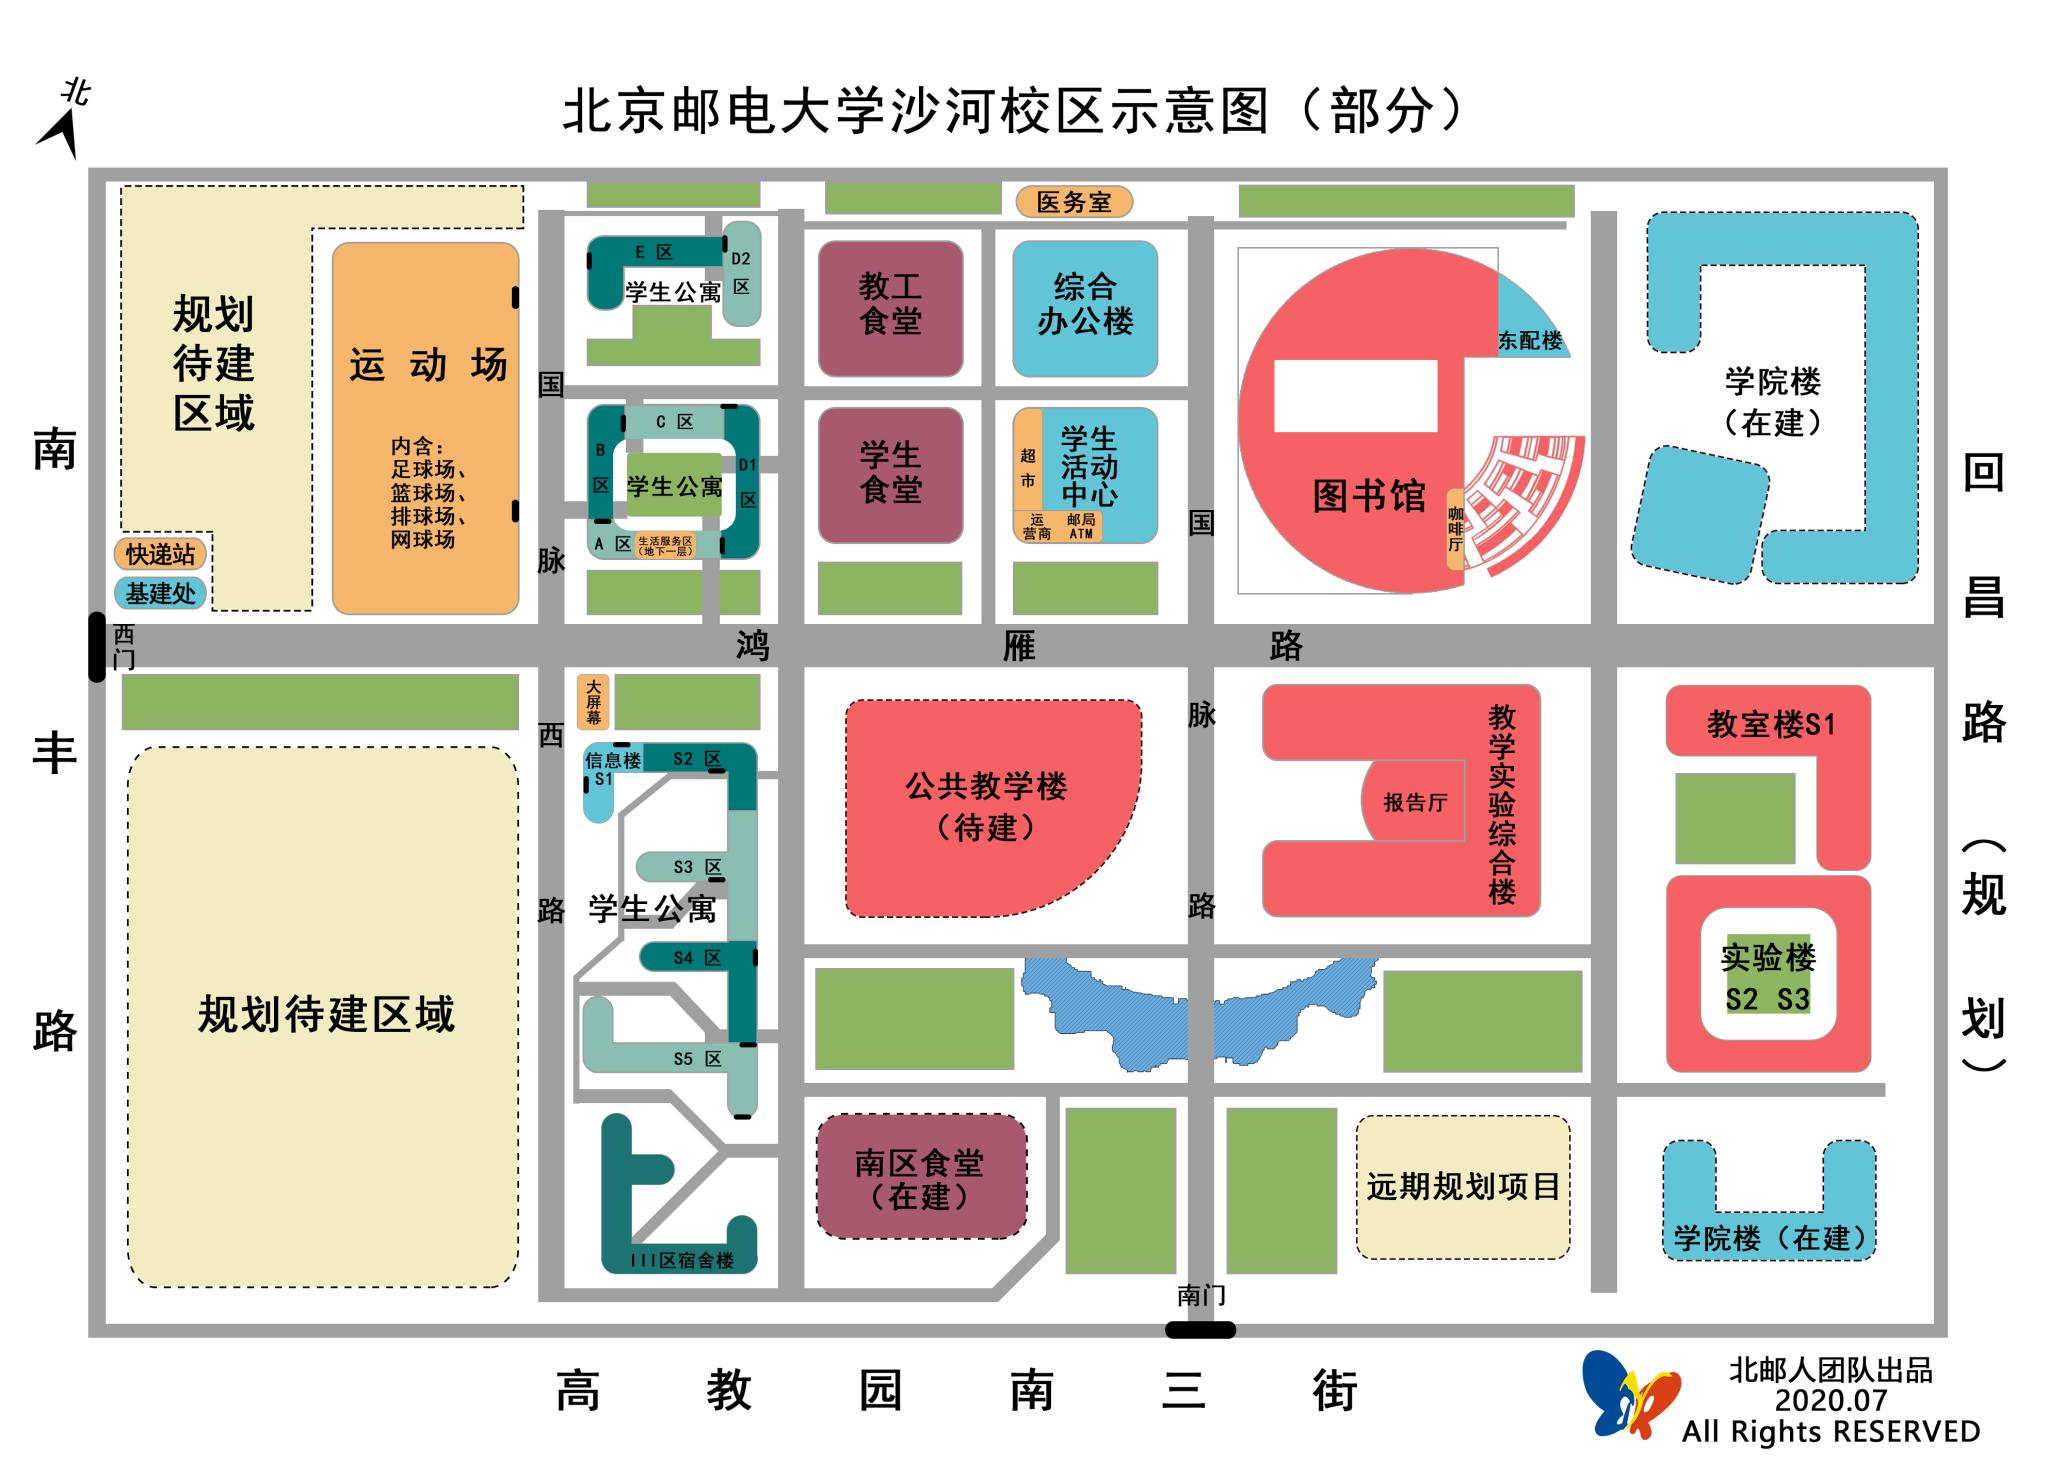
\includegraphics[width=0.80\textwidth]{images/shahe-map.png}
\end{center}

\faq{校园到底有多大?绕一圈要多久?}

很小,真的很小。本部绕一圈仅需10分钟,沙河大概也就20分钟(由于四周还没建设完成,所以(从物理上)根本无法绕圈(笑))。{\small (不过小也有小的好处,比如说可以7:55起床去上8:00的课)}

\faq{我什么时候会从沙河搬到本部?}

学校已经在招生章程中修改了各专业的办学地点。从2022级本科生开始,大部分学院(包括计算机学院在内)的大一会在沙河校区完成,大二至大四均会在校本部就读。\footnote{可在\href{https://zsb.bupt.edu.cn/info/1005/1720.htm}{此}查看各专业办学地点}

\faq{学校现在疫情管控严吗?能不能出去玩啊?}

根据学校目前的政策,出入校采取备案制(但疫情严重时会改为审批制,需要导员同意),不隔夜的情况下自动审批,大家白天出校门应该是没问题啦!关于疫情防控,现在学校内主要措施是进出建筑要戴口罩、测体温和扫二维码,部分食堂的桌子上有隔板,建议大家错位就餐哦(当然也不强制)。上课、体育锻炼和取快递外卖不受影响。

当然,入学后一定会有每日填报信息,大家不要忘哦。虽然也有自动打卡脚本,不过目前严抓,大家还是动动小手自己打卡吧~

\faq{有校车吗?免费吗?}

有,校车往返本部和沙河,但只在工作日安排。学期开始后可以在学校公众号上查询具体班次。由于校车要优先服务老师和本部学生,所以有可能会没有位子。有部分时段的校车需要提前在公众号上预约。

理论上车费5元,比地铁便宜,现在由于刷卡机故障,无需付费。正常情况下需用时35-55分钟,相较于地铁会更快一点,不过昌平线南延段修好以后就不一定了。

\faq{寒暑假我可以住在学校吗?}

目前由于学校规划调整,两个校区寒暑假都不再封校,但受疫情影响可能难以通过假期留校审批。另需支付住宿费。(以届时通知为准)
